\documentclass[11pt,oneside]{article}
\input{coursHeadings}

\usepackage[%
    pdftitle={TD Statique},
    pdfauthor={Xavier Pessoles},
    colorlinks=true,
    linkcolor=blue,
    citecolor=magenta]{hyperref}



% \makeatletter \let\ps@plain\ps@empty \makeatother
%% DEBUT DU DOCUMENT
%% =================
\sloppy
\hyphenpenalty 10000

\newcommand{\Pointilles}[1][3]{%
\multido{}{#1}{\makebox[\linewidth]{\dotfill}\\[\parskip]
}}


\begin{document}


\newboolean{prof}
\setboolean{prof}{false}
%------------- En tetes et Pieds de Pages ------------
\pagestyle{fancy}
\renewcommand{\headrulewidth}{0pt}

\fancyhead{}
\fancyhead[L]{%
\begin{minipage}[c]{1.6cm}

\includegraphics[width=1.4cm]{png/logo_jh_ptsi.png}%
\end{minipage}
\rule{2cm}{.5pt}
}

\fancyhead[C]{\rule{12cm}{.5pt}}

\fancyhead[R]{%
\begin{minipage}[c]{3cm}
\begin{flushright}
\footnotesize{\textit{\textsf{Sciences Industrielles\\ pour l'Ingénieur}}}%
\end{flushright}
\end{minipage}
}

\renewcommand{\footrulewidth}{0.2pt}

\fancyfoot[C]{\footnotesize{\bfseries \thepage}}
\fancyfoot[L]{\footnotesize{2011 -- 2012} \\ X. \textsc{Pessoles}}
\ifthenelse{\boolean{prof}}{%
\fancyfoot[R]{\footnotesize{TD -- CI 3 : Statique -- P}}
}{%
\fancyfoot[R]{\footnotesize{TD -- CI 3 : Statique}}
}


%\begin{center}
%\textit{Centre d'intérêt}
%\end{center}

\begin{center}
 \huge\textsc{CI 3 -- Statique : Modélisation, prévision et vérification du comportement statique des systèmes}
\end{center}

\begin{center}
 \LARGE\textsc{Chapitre 2 -- Principe Fondamental de la Statique} 
\end{center}

%\setcounter{paragraph}{0}
\vspace{.5cm}

\begin{theo}
\textbf{Principe fondamental de la statique -- PFS}

On note $S$ un système matériel à l'équilibre et $\overline{S}$ le milieu extérieur à ce système.

$S$ est à l'équilibre par rapport à un repère galiléen $\mathcal{R}$ si $\forall M \in S$, $\left[\dfrac{d\vect{OM}}{dt}\right]_{\mathcal{R}}=\vect{0}$.

Si $S$ est à l'équilibre, alors : 
$$
\left\{ \mathcal{T} \left( \overline{S} \rightarrow  S\right)\right\} =\{0\}
$$

$\left\{ \mathcal{T}\left( \overline{S} \rightarrow  S\right)\right\}$ désigne la somme des actions mécaniques agissant sur $S$.
\end{theo}

\begin{theo}
\textbf{Équations vectorielles du PFS}

De l'écriture sous forme de torseurs découle deux théorèmes.

Théorème de la résultante statique :
$$
\vectf{\overline{S}}{S}=\vect{0}
$$

Théorème du moment statique au point M :
$$
\vectm{M}{\overline{S}}{S}=\vect{0}
$$

Deux ces 2 équations vectorielles en 3 dimension, on peut donc déduire un système à 6 équations.
\end{theo}

\begin{methode}
\textbf{Détermination des inconnues de liaisons}
\begin{enumerate}
\item Choisir une pièce ou un ensemble de pièce à isoler.
\item Faire le bilan des torseurs des actions mécaniques \textbf{extérieures} au système.
\item Déplacer les torseurs en un même point.
\item Appliquer le PFS appliqué au \textbf{système isolé} en un \textbf{point}.
\item Résoudre le système si le nombre d'inconnues est inférieur ou égal au nombre d'équations.
\item Faire l'application numérique.
\end{enumerate}
\end{methode}

\begin{minipage}[c]{.45\linewidth}
\begin{center}
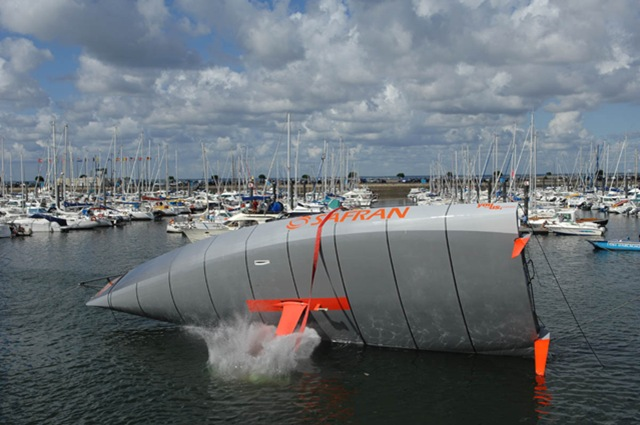
\includegraphics[width=.8\linewidth]{png/safran}

\textit{Safran... du SAFRAN (Skipper Marc Guillemot)}
\end{center}
\end{minipage} \hfill
\begin{minipage}[c]{.45\linewidth}
\begin{center}
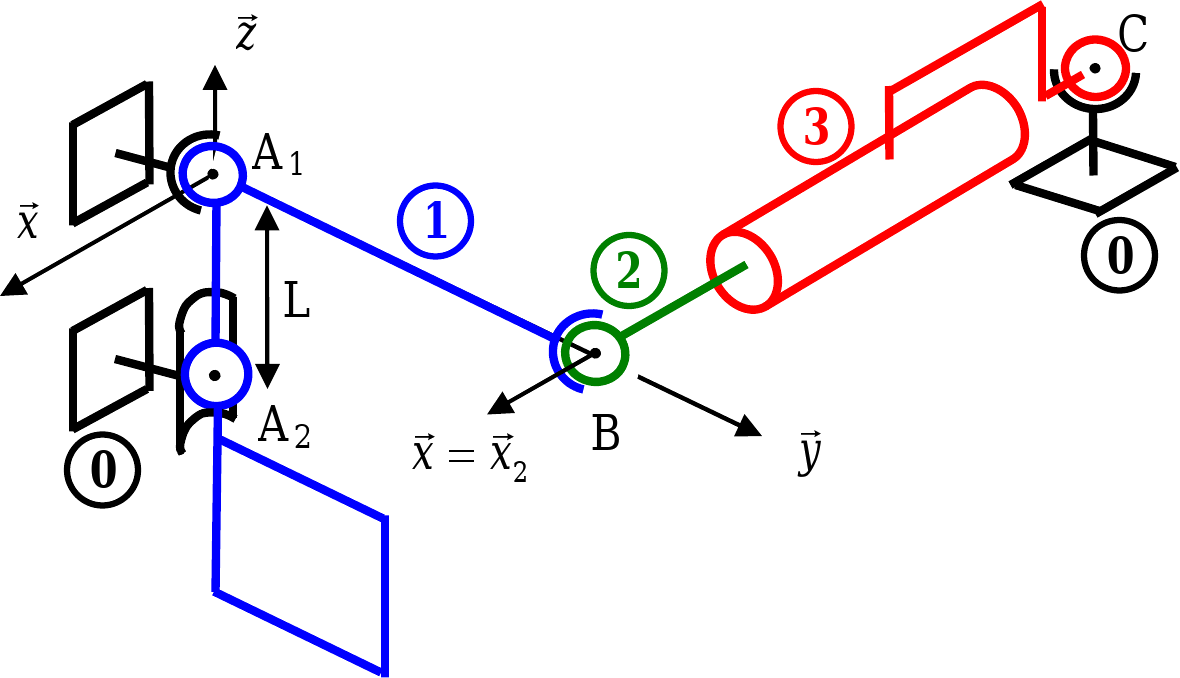
\includegraphics[width=\linewidth]{png/safran2}

\textit{Schéma d'architecture}
\end{center}
\end{minipage}

\vspace{.5cm}

Le safran d'un voilier lui permet de se diriger. Dans le cas du pilote hydraulique du laboratoire, l'angle du safran est asservi afin de pouvoir maintenir un cap, en tenant compte des aléas extérieurs (courants marins, vents violents...). Le safran est actionné par un vérin hydraulique, la pièce 2 étant relié à la tige du vérin et la pièce 3 constituant le corps du vérin. La pièce 1 représente le safran sur lequel agit la pression de l'eau $p$, perpendiculairement au plan du safran. 

L'objectif de l'étude est de calculer les efforts dans les liaisons dans le but ultérieur de dimensionner le vérin hydraulique et les éléments mécaniques assurant les liaisons (éléments roulants ou coussinets). 

\vspace{.5cm}


\setcounter{paragraph}{0}

\begin{minipage}[c]{.6\linewidth}


On donne : 
\begin{itemize}
\item $\vect{A_1B}=h\vect{y}$
\item $\vect{CB}=\lambda\vect{x}$
\end{itemize}

\paragraph{}
\textit{Tracer le graphe de structure associé au système.}

NB : il serait possible d'écrire la loi Entrée -- Sortie liant la vitesse de déploiement du vérin à la vitesse de rotation du safran.

\paragraph{}
\textit{Sur le graphe d'architecture du système indiquer par des flèches les actions mécaniques agissant sur chacune des pièces.}

Par la suite, on négligera l'action de la pesanteur sur les pièces 2 et 3. 

\end{minipage} \hfill
\begin{minipage}[c]{.35\linewidth}
\begin{center}
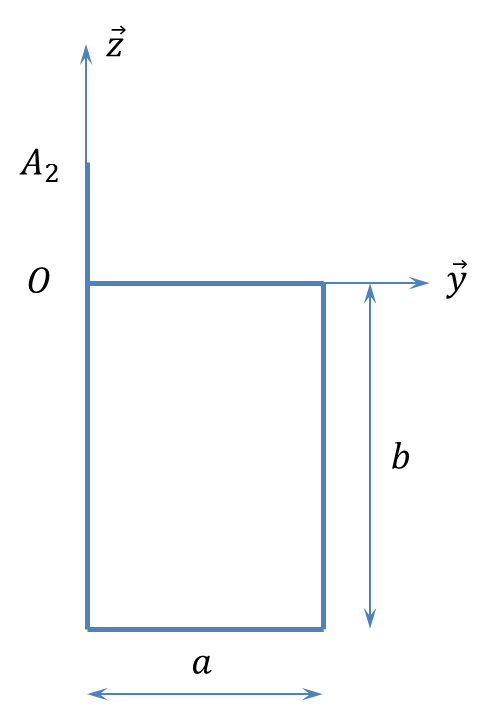
\includegraphics[width=.8\linewidth]{png/safran3}
\end{center}
\end{minipage}

\vspace{.5cm}

\paragraph{}
\textit{Déterminer le torseur d'action mécanique de l'eau sur le gouvernail au point $A_2$. On considèrera que $\vect{OA_2}=\vect{0}$. On négligera l'épaisseur du safran.} 

\paragraph{}
\textit{Après avoir isolé le solide 1, appliquer le principe fondamental de la statique au point $A_1$.}

\paragraph{}
\textit{Quelles inconnues peuvent être déterminées ? Aurait-on pu le prévoir ?}

\paragraph{}
\textit{Après avoir isolé l'ensemble $\{2+3\}$, appliquer le principe fondamental de la statique au point $B$.}


\paragraph{}
\textit{Quelles inconnues ont pu être déterminées ?}


\paragraph{}
\textit{Déterminer l'effort à délivrer par le vérin pour supporter la pression de l'eau sur le safran.}

\paragraph{}
\textit{Déterminer alors la pression à délivrer par le vérin en fonction d'une section $S$.}


\end{document}